\documentclass[11pt,a4paper]{article}

\usepackage[utf8]{inputenc}
\usepackage[T1]{fontenc}
\usepackage[spanish]{babel}
\usepackage{geometry}
\usepackage{graphicx}
\usepackage{array,tabularx,makecell}
\usepackage[table]{xcolor}
\usepackage{fancyhdr,titlesec,helvet,ragged2e,enumitem,setspace}
\usepackage{booktabs,alltt,amsmath,float,placeins,needspace}
\usepackage{xurl}
\usepackage{hyperref}
\usepackage{caption}
\raggedbottom
\renewcommand{\familydefault}{\sfdefault}
\geometry{a4paper,left=3.0cm,right=3.0cm,top=2.35cm,bottom=2.35cm,
  headheight=1.9cm,headsep=0.45cm}
\setlength{\parindent}{0pt}
\setlength{\parskip}{0.22em}
\setlength{\emergencystretch}{2em}
\setlength{\tabcolsep}{6pt}
\renewcommand{\arraystretch}{1.08}
\definecolor{headerblue}{RGB}{19,93,126}
\definecolor{rowlight}{RGB}{205,235,248}
\definecolor{borderblue}{RGB}{64,160,206}
\newcolumntype{L}[1]{>{\RaggedRight\arraybackslash}p{#1}}
\newcolumntype{Y}{>{\RaggedRight\arraybackslash}X}
\newcommand{\cab}[1]{\textbf{\textcolor{white}{#1}}}
\newcommand{\tabestilo}{\arrayrulecolor{borderblue}\setlength{\arrayrulewidth}{0.75pt}\renewcommand{\arraystretch}{1.2}}
\graphicspath{{figures/}{assets/}}
\hypersetup{colorlinks=true,linkcolor=headerblue,citecolor=headerblue,urlcolor=headerblue,
  pdftitle={Reporte Técnico APE 004: Modelo SIR en Java y NetLogo},
  pdfauthor={Richard Ariel Chamba Santin}}
\captionsetup{font=small,labelfont=bf,skip=6pt}
\addto\captionsspanish{\renewcommand{\tablename}{Tabla}}
\setlist{itemsep=0.25em,topsep=0.35em,leftmargin=*}
\pagestyle{fancy}
\fancyhf{}
\fancyhead[L]{
\includegraphics[height=1.35cm]{reporte_tecnico_overleaf_logo.png}}
\fancyhead[R]{\vspace{0.1cm}\small FEIRNNR - Carrera de Computación}
\fancyfoot[C]{\small\thepage}
\renewcommand{\headrulewidth}{0.5pt}
\renewcommand{\footrulewidth}{0pt}
\makeatletter
\renewcommand{\headrule}{{\color{gray!65}\hrule width\headwidth height\headrulewidth\vskip-\headrulewidth}}
\makeatother
\titleformat{\section}{\bfseries\fontsize{15}{17}\selectfont}{\thesection.}{0.8em}{}
\titlespacing*{\section}{0pt}{1.0ex}{0.4ex}
\titleformat{\subsection}{\bfseries\fontsize{12}{14}\selectfont}{\thesubsection.}{0.7em}{}
\titlespacing*{\subsection}{0pt}{1.0ex}{0.4ex}

\begin{document}
\thispagestyle{fancy}
\vspace*{0.15cm}
\begin{center}
{\bfseries\fontsize{23}{26}\selectfont
Reporte Técnico de Actividades\\
Práctico-Experimentales Nro. 004\par}
\end{center}

\section{Datos de Identificación del Estudiante y la Práctica}
\begin{tabularx}{\textwidth}{|L{0.43\textwidth}|Y|}
\hline
\textbf{Nombre del estudiante(s)} & Richard Ariel Chamba Santin \\ \hline
\textbf{Asignatura} & Simulación \\ \hline
\textbf{Ciclo} & 5 \\ \hline
\textbf{Unidad} & U1: Introducción a la Simulación \\ \hline
\makecell[l]{\textbf{Resultado de aprendizaje}\\\textbf{de la unidad}} & R1. Aplica análisis estadísticos de los datos de la Simulación para mejorar la calidad de los resultados, bajo los principios de solidaridad, transparencia, responsabilidad y honestidad. \\ \hline
\textbf{Práctica Nro.} & 004 \\ \hline
\textbf{Título de la Práctica} & Análisis comparativo de herramientas de simulación mediante un modelo común \\ \hline
\textbf{Nombre del Docente} & José O. Guamán Q. \\ \hline
\textbf{Fecha de la práctica} & 22 y 23 de octubre de 2026 \\ \hline
\textbf{Horario} & \makecell[l]{Jueves 10h30 a 11h30\\Viernes 07h30 a 09h30} \\ \hline
\textbf{Lugar} & Aula \\ \hline
\textbf{Tiempo planificado en el Sílabo} & 3 horas \\ \hline
\end{tabularx}

\vspace{0.4cm}
Los datos de la práctica corresponden a la Guía APE Nro. 004 del docente~\cite{guia}.
Las corridas reproducibles y las figuras de este informe se prepararon el 24 de octubre de 2026.
\newpage

\section{Objetivo(s) de la Práctica}
Comparar diferentes lenguajes y plataformas para implementar un modelo común de simulación~\cite{guia}.
\begin{enumerate}
  \item Implementar un modelo epidemiológico SIR con las mismas reglas y parámetros en distintas herramientas.
  \item Comparar la sintaxis, la facilidad de implementación y las opciones de visualización.
  \item Identificar el ámbito de aplicación de cada herramienta y explicar las diferencias producidas por el azar.
\end{enumerate}
En el proyecto se desarrollaron y ejecutaron las versiones de \textbf{Java y NetLogo}.
La guía también solicita Python/SimPy; esa versión no se implementó y, por tanto, no se presentan resultados experimentales de ella.

\section{Materiales y reactivos}
\begin{itemize}
  \item Guía de Actividades Práctico-Experimentales Nro. 004 y código fuente del proyecto.
  \item Modelo SIR con población inicial de 100 personas y estados S, I y R.
  \item Archivos CSV de resultados y de parámetros para el intercambio de información.
  \item Documentación oficial de Java, NetLogo y SimPy como apoyo a las preguntas conceptuales.
\end{itemize}

\section{Equipos y herramientas}
\begin{itemize}
  \item Computador con sistema operativo Linux y editor de código.
  \item OpenJDK 27 para compilar y ejecutar Java; se utilizó \texttt{--release 11} para generar clases compatibles con Java 11.
  \item NetLogo 7.0.4, con la extensión \texttt{csv}; se utilizó su interfaz y el mismo modelo en ejecución sin interfaz para exportar los datos.
  \item Git y GitHub para el control de versiones y la publicación del proyecto.
  \item Python con Matplotlib para reproducir las figuras a partir de los CSV. Este uso es de presentación de datos; no constituye una implementación SIR en Python/SimPy.
  \item \LaTeX{} para la redacción del informe y Tectonic para compilar el PDF.
\end{itemize}

\section{Link Repositorio}
\url{https://github.com/RichardChambaS/Ape4_Simulacion}

\newpage
\section{Procedimiento / Metodología Ejecutada}

\subsection{Fundamento teórico y delimitación del modelo}
El modelo SIR representa la propagación de una infección en una población dividida en susceptibles ($S$), infectados ($I$) y recuperados ($R$). En esta práctica la población es cerrada: no se incorporan nacimientos, muertes ni reinfecciones. Por ello se conserva~\cite{guia}:
\[
N=S(t)+I(t)+R(t).
\]
La guía presenta el sistema diferencial:
\begin{align*}
\frac{dS}{dt}&=-\beta\frac{SI}{N}, &
\frac{dI}{dt}&=\beta\frac{SI}{N}-\gamma I, &
\frac{dR}{dt}&=\gamma I.
\end{align*}
Estas ecuaciones explican el flujo $S\rightarrow I\rightarrow R$. Para la implementación se eligió la alternativa discreta por agentes permitida por la guía; no se resolvió numéricamente el sistema diferencial.
En el código, $\beta$ se utiliza como probabilidad de infección por contacto y $\gamma$ como probabilidad de recuperación por paso.

El número reproductivo básico de referencia de la guía se escribe aquí como
$\mathcal{R}_0=\beta/\gamma=0{,}30/0{,}10=3$ para distinguirlo del conteo inicial de recuperados, $R(0)=0$. Es una referencia del modelo teórico; no se estimó empíricamente ese número en las corridas por agentes.

\begin{table}[H]
\centering\tabestilo
\begin{tabularx}{\textwidth}{|Y|c|}
\hline\rowcolor{headerblue}\cab{Parámetro de la corrida base} & \cab{Valor} \\ \hline
Población $N$ & 100 \\ \hline
\rowcolor{rowlight}Susceptibles iniciales $S(0)$ & 95 \\ \hline
Infectados iniciales $I(0)$ & 5 \\ \hline
\rowcolor{rowlight}Recuperados iniciales $R(0)$ & 0 \\ \hline
Probabilidad de contagio por contacto $\beta$ & $0{,}30$ \\ \hline
\rowcolor{rowlight}Probabilidad de recuperación por paso $\gamma$ & $0{,}10$ \\ \hline
Horizonte de simulación & 100 pasos \\ \hline
\rowcolor{rowlight}Semilla para reproducir cada implementación & 42 \\ \hline
\end{tabularx}
\caption{Configuración común. La semilla se añadió para reproducir las corridas; los demás valores proceden de la Guía APE 004.}
\label{tab:parametros}
\end{table}

\subsection{Reglas comunes y actualización de los estados}
Se definió una misma regla para Java y NetLogo: cada persona que estaba infectada al comenzar un paso selecciona \textbf{un contacto al azar entre las demás personas}. El contacto no depende de la cercanía visual. Si esa persona era susceptible, se intenta infectarla con probabilidad $\beta$. De forma independiente, el infectado puede recuperarse con probabilidad $\gamma$.

Se conservó una copia de los estados al inicio del paso. Los contagios y recuperaciones se anotaron en un estado siguiente y se aplicaron juntos al terminar. De esta manera, quien acaba de infectarse participa en los contactos a partir del siguiente paso. Dos infectados pueden elegir al mismo susceptible, pero esa persona se cuenta una sola vez.

\noindent\begin{minipage}{\textwidth}
\begin{alltt}\small
Inicializar 95 susceptibles, 5 infectados y 0 recuperados
Guardar el estado inicial en t = 0
Para t = 1 hasta 100:
    Copiar los estados de todas las personas
    Para cada persona infectada al inicio del paso:
        Elegir otra persona como contacto, si existe
        Intentar contagiarla con probabilidad \(\beta\)
        Intentar recuperarse con probabilidad \(\gamma\)
    Aplicar los cambios simultáneamente
    Contar y guardar S, I y R
\end{alltt}
\end{minipage}

Una persona puede contagiar y recuperarse en el mismo paso, porque la evaluación usa su estado inicial. Los recuperados conservan su estado hasta el final. Se registró desde $t=0$ hasta $t=100$, con \textbf{101 filas de datos}, incluso cuando ya no quedaban infectados.

\Needspace{8\baselineskip}
\subsection{Implementación de Java con Modelo, Vista y Controlador}
Se organizó el programa en clases para separar las reglas de la simulación, la salida por consola y la escritura de los archivos:
\begin{itemize}
  \item \textbf{Modelo:} \path{src/modelo/Persona.java} define los estados de cada individuo; \path{src/modelo/SimulacionSIR.java} contiene los parámetros, las transiciones y el conteo de la población.
  \item \textbf{Vista:} \path{src/vista/VistaConsola.java} presenta los parámetros, una tabla cada diez pasos, el pico de infectados y el tiempo de cálculo.
  \item \textbf{Controlador:} \path{src/controlador/SimulacionControlador.java} ejecuta el modelo, guarda los CSV y deja una copia de ellos junto al modelo de NetLogo.
  \item \textbf{Entrada:} \path{src/Main.java} inicia el controlador y comunica errores de parámetros o de escritura con mensajes claros.
\end{itemize}
Para generar los datos se ejecutaron estos comandos desde la raíz del proyecto:
{\small
\begin{verbatim}
javac -encoding UTF-8 --release 11 -d build \
  src/Main.java src/modelo/*.java \
  src/vista/*.java src/controlador/*.java
java -cp build Main
\end{verbatim}
}

No basta con editar una constante: es necesario compilar y ejecutar otra vez para que los archivos contengan los resultados del nuevo escenario. La aplicación utiliza \texttt{java.util.Random} con la semilla configurada; una misma semilla y la misma secuencia de llamadas permiten repetir la ejecución de Java~\cite{java}.

\subsection{Integración de resultados y parámetros mediante CSV}
Se implementó el flujo
\[
\text{Java}\;\longrightarrow\;\text{archivos CSV}\;\longrightarrow\;\text{NetLogo}.
\]
Java genera \path{resultados/resultados_java.csv} y copia el archivo en \path{netlogo/resultados_java.csv}. Sus columnas son:
{\small
\begin{verbatim}
tiempo,susceptibles,infectados,recuperados
0,95,5,0
1,92,7,1
\end{verbatim}
}

Además, exporta \path{parametros_java.csv} en ambas carpetas, con la población, los infectados iniciales, beta, gamma, tiempo máximo y semilla. La fila de la corrida base es:
{\small
\begin{verbatim}
poblacion,infectados_iniciales,beta,gamma,tiempo_maximo,semilla
100,5,0.3,0.1,100,42
\end{verbatim}
}

Al pulsar \textbf{ACTUALIZAR JAVA}, NetLogo lee ambos archivos, reinicia su escenario y muestra los parámetros activos. Así se evita comparar un CSV nuevo de Java con una simulación de NetLogo configurada con valores anteriores. La extensión \texttt{csv} proporciona la lectura de las filas como listas de valores~\cite{csv}.

\subsection{Preparación y uso de NetLogo}
Se abrió \path{netlogo/modelo_sir_netlogo.nlogox} en NetLogo 7.0.4. Cada persona se representó como un agente visible: azul si es susceptible, rojo si está infectado y verde si está recuperado. La persona de identificador 0 lleva la etiqueta P0; en la corrida base pertenece a los cinco infectados iniciales.

El procedimiento \texttt{setup} crea la población, aplica la semilla, registra el tiempo inicial y carga los archivos disponibles. El botón \textbf{ACTUALIZAR JAVA} realiza esa sincronización y confirma la cantidad de filas importadas. Luego, \textbf{go} avanza la simulación de NetLogo hasta alcanzar el tiempo máximo; al volver a pulsarlo se interrumpe su ejecución continua.

El deslizador \textbf{PAUSA}, expresado en segundos, regula la espera visual entre pasos. Se conservó el nombre \texttt{PAUSA} en el control y en el código después de comprobar su carga en la interfaz de NetLogo. Su valor inicial actual es cero; aumentarlo ralentiza la animación, sin cambiar las reglas epidemiológicas ni el tiempo simulado.

El movimiento de las figuras es ilustrativo. Se utilizó \texttt{with-local-randomness} para que el azar de sus posiciones y desplazamientos no altere la secuencia utilizada por las reglas SIR. La simulación propia de NetLogo genera su curva por pasos; la curva de Java se importa completa desde el CSV.

\subsection{Obtención de las gráficas de la corrida base}
Se ejecutaron las dos implementaciones con los parámetros de la Tabla~\ref{tab:parametros}. Los datos Java se guardaron en el CSV de resultados. Para el informe se exportó también la lista \texttt{datos-netlogo} del mismo modelo de NetLogo, con 101 registros. Las figuras siguientes se trazaron con Matplotlib a partir de esos archivos, sin sustituir la simulación de NetLogo por un programa de Python.

Se conservaron los datos en \path{reports/data/}; el script \path{reports/scripts/generar_figuras.py} permite regenerar las figuras. Las dos primeras muestran la evolución SIR por herramienta y las tres siguientes comparan el mismo estado entre herramientas.

\begin{figure}[H]
\centering
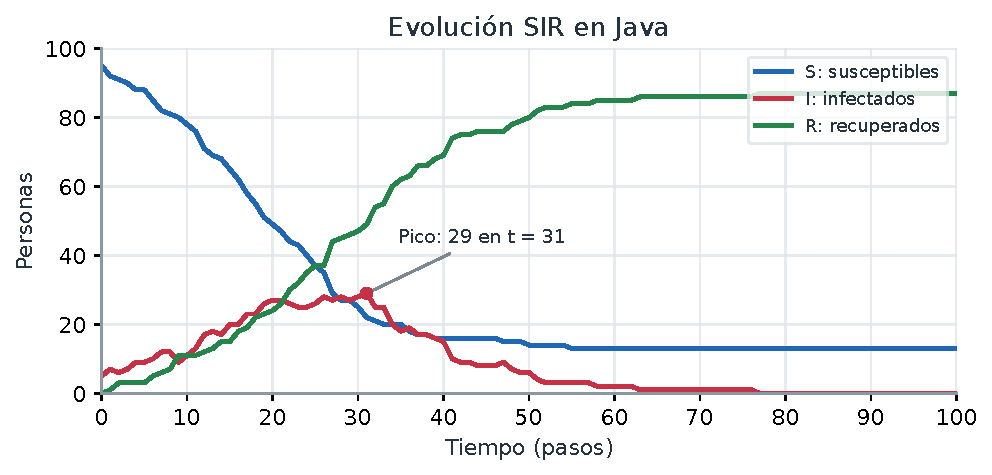
\includegraphics[width=\textwidth]{01_evolucion_java.pdf}
\caption{Evolución SIR obtenida por Java. El máximo de infectados es 29 en $t=31$; en $t=100$ quedan 13 susceptibles y 87 recuperados. Fuente: corrida base de Java.}
\label{fig:java}
\end{figure}

\begin{figure}[H]
\centering
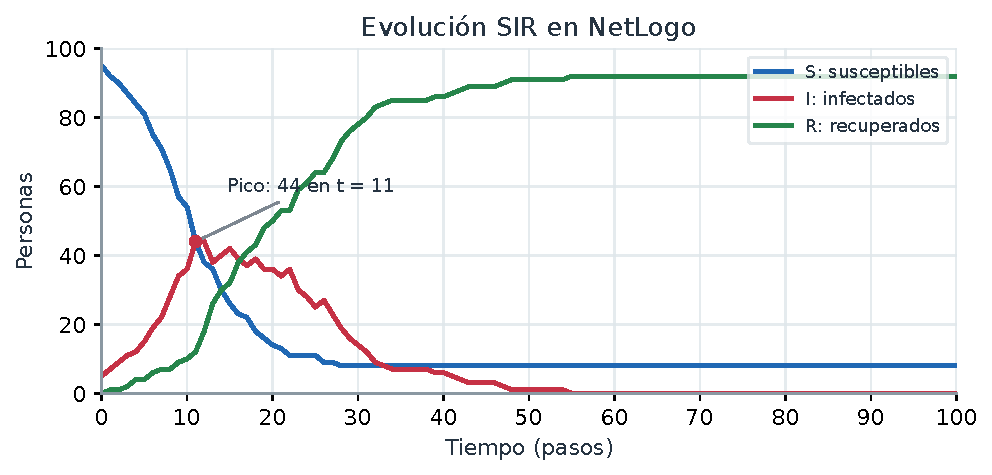
\includegraphics[width=\textwidth]{02_evolucion_netlogo.pdf}
\caption{Evolución SIR calculada por NetLogo. El primer máximo de 44 infectados ocurre en $t=11$; al final quedan 8 susceptibles y 92 recuperados. Fuente: corrida base de NetLogo 7.0.4.}
\label{fig:netlogo}
\end{figure}

\begin{figure}[H]
\centering
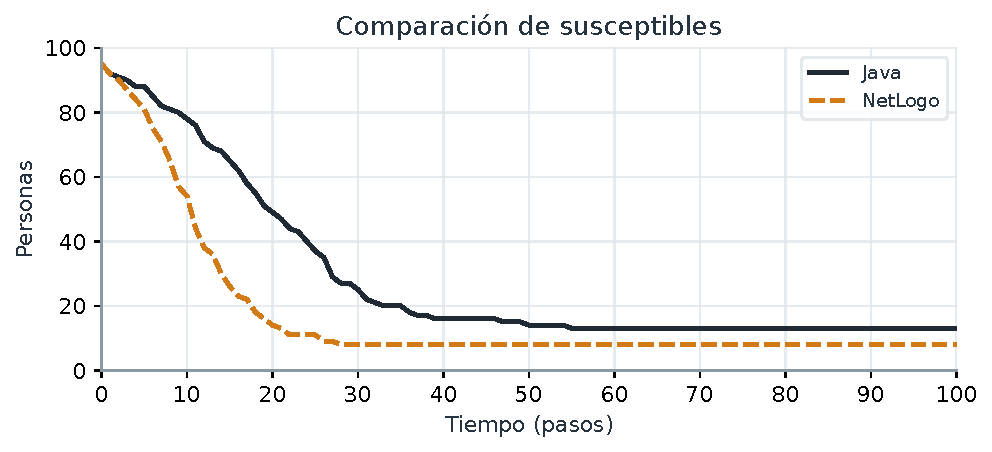
\includegraphics[width=\textwidth]{03_comparacion_susceptibles.pdf}
\caption{Comparación de susceptibles. Ambas series comienzan en 95 y disminuyen; terminan en 13 para Java y 8 para NetLogo. Negro: Java; naranja: NetLogo.}
\label{fig:s}
\end{figure}

\begin{figure}[H]
\centering
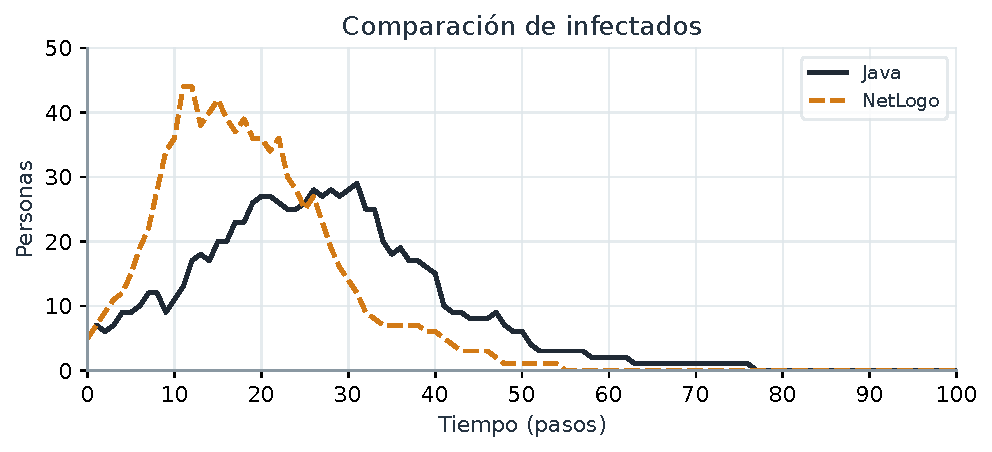
\includegraphics[width=\textwidth]{04_comparacion_infectados.pdf}
\caption{Comparación de infectados. Java alcanza su pico en $t=31$ y NetLogo en $t=11$. Los infectados llegan a cero en $t=77$ y $t=55$, respectivamente.}
\label{fig:i}
\end{figure}

\begin{figure}[H]
\centering
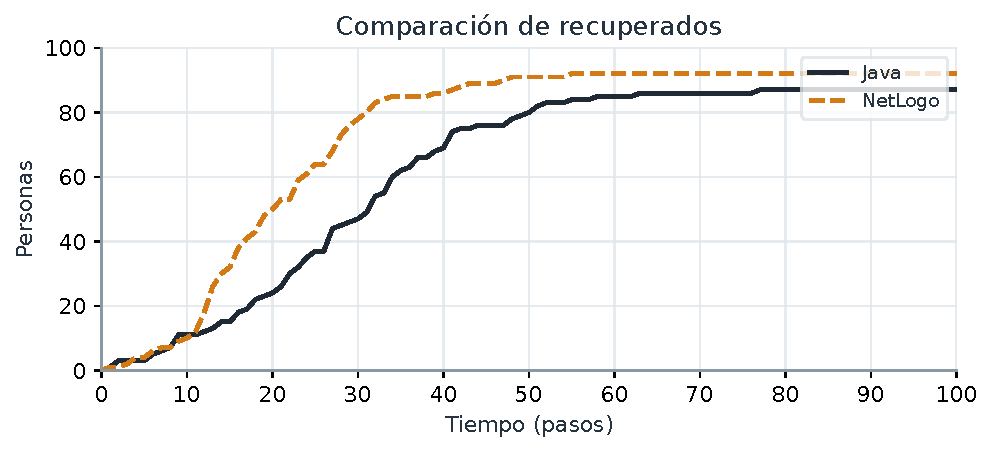
\includegraphics[width=\textwidth]{05_comparacion_recuperados.pdf}
\caption{Comparación de recuperados. Las dos curvas aumentan de forma acumulativa. Al final se registran 87 recuperados en Java y 92 en NetLogo.}
\label{fig:r}
\end{figure}

\subsection{Cambio de parámetros: prueba con recuperación más rápida}
Para comprobar el flujo de actualización se ejecutó también una copia de prueba con \texttt{GAMMA = 0.40}, conservando población, infectados iniciales, beta, horizonte y semilla. Java regeneró los CSV y NetLogo leyó esa configuración antes de ejecutar el nuevo escenario. Esta prueba se realizó por separado; el código principal se mantuvo con $\gamma=0{,}10$.

El procedimiento para repetir una demostración en pantalla es: editar el valor en Java, compilar, ejecutar, pulsar \textbf{ACTUALIZAR JAVA} en NetLogo, comprobar el valor de gamma que aparece en pantalla y pulsar \textbf{go}. El botón lee archivos; la compilación y ejecución de Java se hacen antes, en la terminal.

\begin{figure}[H]
\centering
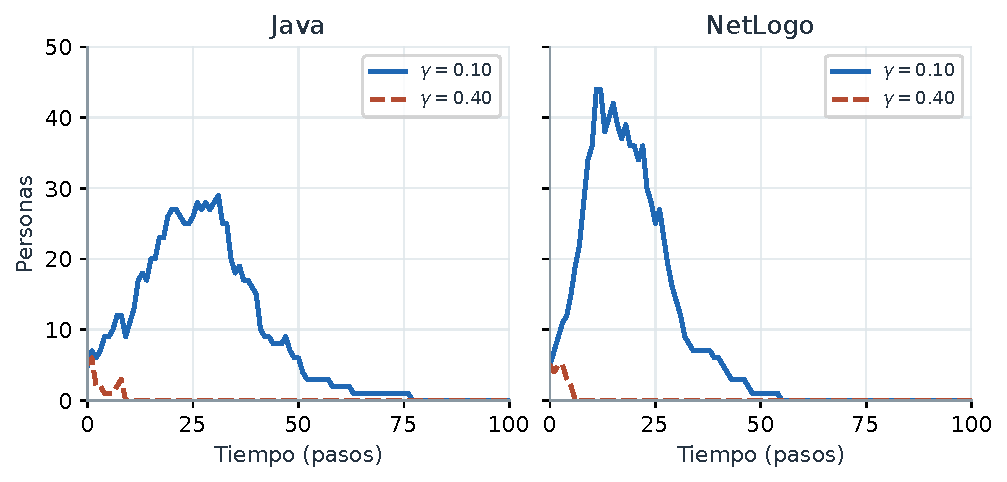
\includegraphics[width=\textwidth]{06_efecto_gamma.pdf}
\caption{Efecto de cambiar $\gamma$ de $0{,}10$ a $0{,}40$ manteniendo los demás parámetros. La recuperación más rápida reduce el brote en las corridas observadas. Cada panel corresponde a una implementación independiente.}
\label{fig:gamma}
\end{figure}

\begin{table}[H]
\centering\tabestilo
\begin{tabularx}{\textwidth}{|Y|c|c|}
\hline\rowcolor{headerblue}\cab{Medida con $\gamma=0{,}40$} & \cab{Java} & \cab{NetLogo} \\ \hline
Pico de infectados & 6 & 5 \\ \hline
\rowcolor{rowlight}Primer tiempo del pico & 1 & 0 \\ \hline
Primer tiempo sin infectados & 9 & 6 \\ \hline
\rowcolor{rowlight}Estado final $(S,I,R)$ & $(89,0,11)$ & $(89,0,11)$ \\ \hline
\end{tabularx}
\caption{Corridas de demostración con gamma $0{,}40$. La coincidencia del estado final no significa que las trayectorias sean idénticas.}
\label{tab:gamma}
\end{table}

\subsection{Verificaciones y tratamiento de entradas inválidas}
Se comprobó en las series exportadas que los conteos fueran enteros no negativos, que $S+I+R=100$ en cada fila, que $S$ no aumentara y que $R$ no disminuyera. También se verificaron el estado inicial, la secuencia de tiempos y la cantidad de registros. Las copias de los CSV en las carpetas de resultados y de NetLogo coincidieron.

Para evitar fallos al modificar parámetros, Java valida la configuración antes de simular o escribir archivos. NetLogo valida las filas importadas y la configuración recibida. Se ejecutaron 16 casos de comprobación en Java y 12 en NetLogo, utilizando copias temporales para no modificar los resultados de la corrida base. Entre los casos revisados estuvieron:
\begin{table}[H]
\centering\tabestilo\small
\begin{tabularx}{\textwidth}{|L{0.35\textwidth}|Y|}
\hline\rowcolor{headerblue}\cab{Caso revisado} & \cab{Comportamiento comprobado} \\ \hline
Una persona y un infectado inicial & No se intenta un contacto inexistente; la persona puede recuperarse. \\ \hline
\rowcolor{rowlight}Ningún infectado o todos infectados & Se conservan conteos válidos y la población total. \\ \hline
Beta y gamma cercanos a 1 & Se acepta $0{,}9999999$, porque es una probabilidad válida. \\ \hline
\rowcolor{rowlight}Tiempo máximo igual a cero & Se guarda únicamente el estado inicial. \\ \hline
Población nula, infectados fuera de rango o probabilidades inválidas & Se informa el parámetro incorrecto; Java no reemplaza los CSV anteriores. \\ \hline
\rowcolor{rowlight}CSV con personas fraccionarias & NetLogo rechaza el archivo con un mensaje; los conteos no se redondean. \\ \hline
\end{tabularx}
\caption{Casos representativos de las verificaciones realizadas. Una fracción es válida para una probabilidad, pero no para contar personas.}
\end{table}
\FloatBarrier

\section{Resultados esperados}
De acuerdo con la Guía APE 004, se espera disponer de un modelo común en NetLogo, Python/SimPy y Java; archivos CSV de Python y Java; gráficas de susceptibles, infectados y recuperados; visualización de esos datos en NetLogo; y un análisis de ventajas, limitaciones y diferencias atribuibles al azar~\cite{guia}.

En el alcance realizado se obtuvieron las versiones Java y NetLogo, la integración de Java por CSV, cinco gráficas de comparación y una prueba adicional de cambio de parámetros. La implementación Python/SimPy y su CSV siguen fuera del alcance ejecutado. El video de demostración indicado en la evaluación no se adjunta a este documento.

\section{Resultados}
\subsection{Resumen de la corrida base}
\begin{table}[H]
\centering\tabestilo
\begin{tabularx}{\textwidth}{|Y|c|c|}
\hline\rowcolor{headerblue}\cab{Medida} & \cab{Java} & \cab{NetLogo} \\ \hline
Registros de tiempo & 101 & 101 \\ \hline
\rowcolor{rowlight}Máximo de infectados & 29 & 44 \\ \hline
Primer tiempo del máximo & 31 & 11 \\ \hline
\rowcolor{rowlight}Primer tiempo con $I=0$ & 77 & 55 \\ \hline
Susceptibles en $t=100$ & 13 & 8 \\ \hline
\rowcolor{rowlight}Infectados en $t=100$ & 0 & 0 \\ \hline
Recuperados en $t=100$ & 87 & 92 \\ \hline
\rowcolor{rowlight}Población total conservada & 100 & 100 \\ \hline
\end{tabularx}
\caption{Resultados de una corrida por herramienta: $N=100$, $\beta=0{,}30$, $\gamma=0{,}10$ y semilla 42.}
\label{tab:resultados}
\end{table}
Se conservaron todos los tiempos hasta 100 aunque la infección desapareciera antes. Por eso, a partir de $t=77$ en Java y de $t=55$ en NetLogo, las series permanecen constantes. Los datos son observaciones de corridas individuales; no son promedios ni intervalos de confianza.

\subsection{Comparación de la experiencia de implementación}
\begin{table}[H]
\centering\tabestilo\footnotesize
\setlength{\tabcolsep}{4pt}
\begin{tabularx}{\textwidth}{|L{0.19\textwidth}|Y|L{0.15\textwidth}|Y|}
\hline\rowcolor{headerblue}\cab{Característica} & \cab{NetLogo} & \cab{Python/SimPy} & \cab{Java} \\ \hline
Facilidad de implementación & Reglas de agentes y gráficas dentro del mismo entorno. & No implementado. & Fue necesario crear clases, arreglos y exportación. \\ \hline
\rowcolor{rowlight}Manejo de agentes & Cada persona es una tortuga con estado y color. & No evaluado. & Cada persona es un objeto con un estado enumerado. \\ \hline
Generación de datos & Genera su serie y lee los CSV externos. & Sin datos. & Genera resultados y parámetros en CSV. \\ \hline
\rowcolor{rowlight}Visualización & Se observaron movimiento, conteos y cinco gráficas. & No evaluado. & Se usó consola; las curvas se visualizaron en NetLogo. \\ \hline
Flexibilidad & Fue posible cambiar reglas y observar sus efectos en los agentes. & No evaluado. & MVC permitió separar el cálculo de la salida y los archivos. \\ \hline
\rowcolor{rowlight}Tiempo de ejecución & El monitor acumula actualizaciones SIR y excluye animación y pausa. & Sin medición. & La consola mide cálculo y conteos, antes de escribir el CSV. \\ \hline
Integración con otras herramientas & La extensión CSV permitió importar la serie de Java. & No evaluado. & Se copiaron automáticamente resultados y parámetros a NetLogo. \\ \hline
\end{tabularx}
\caption{Comparación basada en lo realizado. Los tiempos de Java y NetLogo abarcan tareas diferentes; no se efectuó una comparación controlada de rendimiento.}
\label{tab:experiencia}
\end{table}
\FloatBarrier

\section{Análisis de Resultados}
\subsection{Evolución de Java y NetLogo}
En la Figura~\ref{fig:java}, Java inicia con 95 susceptibles, 5 infectados y ningún recuperado. Los infectados aumentan hasta 29 en el paso 31 y luego disminuyen hasta cero en el paso 77. Al final, 87 personas han pasado al estado recuperado y 13 nunca se infectaron.

En la Figura~\ref{fig:netlogo}, el brote crece antes: NetLogo alcanza 44 infectados en el paso 11. La infección desaparece en el paso 55 y termina con 92 recuperados y 8 susceptibles. La diferencia del pico es de 15 personas, y el primer máximo aparece 20 pasos antes que en Java. Esto describe estas dos corridas; no demuestra un comportamiento general de una herramienta frente a la otra.

\subsection{Interpretación de las tres comparaciones}
La comparación de susceptibles (Figura~\ref{fig:s}) muestra curvas descendentes: una persona solo puede salir de S hacia I. La serie de NetLogo desciende más rápido al comienzo y termina con cinco susceptibles menos que Java.

La comparación de infectados (Figura~\ref{fig:i}) concentra la principal diferencia temporal. Los máximos tienen distinta altura y aparecen en momentos distintos, aunque las reglas y los valores de beta y gamma sean iguales. El estado I recibe personas por contagio y pierde personas por recuperación; su forma depende de ambos procesos aleatorios.

La comparación de recuperados (Figura~\ref{fig:r}) muestra crecimiento acumulativo: nadie sale del estado R. Como en las dos corridas $I(100)=0$, los recuperados finales representan a todas las personas que estuvieron infectadas, incluidos los cinco infectados iniciales. Sus cantidades equivalen al 87\,\% de la población en Java y al 92\,\% en NetLogo.

\subsection{Efecto del azar y de la recuperación}
Se mantuvo el orden de actualización de los agentes y la misma regla de contactos para comparar el mismo modelo. Sin embargo, Java y NetLogo producen secuencias aleatorias diferentes: usar el mismo número como semilla reproduce cada implementación, pero no sincroniza sus sorteos. Por eso se esperan trayectorias distintas.

En la prueba con $\gamma=0{,}40$ (Figura~\ref{fig:gamma}), la recuperación por paso fue más probable y las infecciones desaparecieron pronto: en $t=9$ para Java y en $t=6$ para NetLogo. Los máximos fueron 6 y 5, respectivamente. La coincidencia final en $(89,0,11)$ muestra que también pueden obtenerse conteos finales iguales mediante trayectorias distintas.

Para afirmar diferencias sistemáticas sería necesario ejecutar varias semillas y comparar distribuciones, medias e intervalos de confianza. Este informe presenta una corrida base y un escenario de demostración por herramienta; las comprobaciones de entradas inválidas no sustituyen a las réplicas estadísticas.

\subsection{Alcance de la integración}
La separación del cálculo y la visualización permitió conservar los datos originales, verificar los conteos y regenerar las gráficas. El archivo de parámetros resolvió el desfase que aparecía al cambiar gamma en Java sin actualizar la configuración de NetLogo. El flujo sigue siendo por archivos: primero se ejecuta Java y después se actualiza NetLogo.

La comparación solicitada por la guía se completó para Java y NetLogo. Python/SimPy no se implementó, por lo que no se atribuyen ventajas experimentales ni tiempos de ejecución a esa herramienta.

\section{Preguntas de Control}
\begin{enumerate}
\item \textbf{\textquestiondown{}Qué representa el modelo SIR?}
\par Representa la evolución de una población durante la propagación de una infección. Describe cómo las personas pasan de susceptibles a infectadas y después a recuperadas. En la variante usada no hay reinfección, nacimientos ni muertes, por lo que la población total permanece constante~\cite{guia}.

\item \textbf{\textquestiondown{}Qué representan los estados S, I y R?}
\par S representa a quienes todavía pueden infectarse; I, a quienes están infectados y pueden transmitir la infección; R, a quienes se recuperaron y no vuelven a infectarse en este modelo. Sus conteos satisfacen $S+I+R=N$ en cada tiempo~\cite{guia}.

\item \textbf{\textquestiondown{}Qué función cumplen los parámetros $\beta$ y $\gamma$?}
\par $\beta$ controla la transmisión y $\gamma$ la recuperación. En nuestro programa, un contacto con un susceptible produce infección con probabilidad $\beta$, y cada infectado se recupera en un paso con probabilidad $\gamma$. La corrida base utiliza $0{,}30$ y $0{,}10$; al aumentar gamma a $0{,}40$ se observó una recuperación más rápida.

\item \textbf{\textquestiondown{}Por qué es importante utilizar los mismos parámetros en las tres herramientas?}
\par Para comparar el mismo escenario. Si una herramienta utiliza otra población, otra probabilidad o una duración distinta, las diferencias de las curvas podrían deberse a esa configuración. En este proyecto, Java exporta los parámetros y NetLogo los lee antes de simular, de modo que la comparación ejecutada conserva los mismos valores.

\item \textbf{\textquestiondown{}Por qué Python, Java y NetLogo pueden producir resultados diferentes utilizando el mismo modelo?}
\par Porque las simulaciones usan números pseudoaleatorios, y cada herramienta puede generar secuencias diferentes. También influye el orden en que se hacen los sorteos y se aplican los cambios. Mantener la semilla permite repetir una corrida dentro de cada implementación, pero no obliga a que los generadores de lenguajes distintos produzcan la misma trayectoria. Java documenta esta reproducibilidad para la misma semilla y secuencia de llamadas~\cite{java}.

\item \textbf{\textquestiondown{}Qué ventajas ofrece NetLogo para representar sistemas basados en agentes?}
\par Incluye agentes, espacio y controles visuales dentro del mismo entorno~\cite{netlogo}. En nuestro caso fue posible representar cada persona, observar su color y contar S, I y R mientras se construían las gráficas. Esto facilitó relacionar las reglas individuales con el comportamiento del conjunto.

\item \textbf{\textquestiondown{}Qué ventajas ofrece SimPy para desarrollar simulaciones basadas en eventos?}
\par SimPy permite describir procesos que esperan y se reanudan mediante eventos, administrar el tiempo de la simulación y representar recursos compartidos con capacidad limitada~\cite{simpy}. Es útil, por ejemplo, para clientes que esperan atención o tareas que compiten por un recurso. Esta respuesta es conceptual: no se ejecutó una versión del modelo con SimPy.

\item \textbf{\textquestiondown{}Qué ventajas ofrece Java para implementar modelos de simulación?}
\par En esta práctica permitió representar las personas mediante objetos, definir sus estados de forma explícita y organizar el programa con MVC. También permitió controlar los sorteos, validar la configuración y exportar los datos sin depender de la interfaz de NetLogo. La separación entre modelo, vista y controlador facilitó localizar cada responsabilidad.

\item \textbf{\textquestiondown{}Qué función cumple el archivo CSV en la integración Python/Java $\rightarrow$ NetLogo?}
\par Transporta los resultados calculados externamente para que NetLogo los lea y grafique~\cite{csv}. Aquí el CSV de Java contiene tiempo, susceptibles, infectados y recuperados; otro CSV lleva los parámetros del escenario. NetLogo importa esos datos y conserva su propia simulación como una serie independiente para la comparación.

\item \textbf{\textquestiondown{}Qué ventajas presenta separar la generación de datos de la visualización?}
\par Permite ejecutar y comprobar el cálculo por separado, conservar una evidencia de los resultados y representar el mismo archivo en otras herramientas. También facilita repetir un escenario o cambiar el formato de las gráficas sin modificar las reglas de contagio y recuperación. En nuestro proyecto se pudo regenerar el informe a partir de los CSV guardados.
\end{enumerate}
\FloatBarrier

\section{Conclusiones}
\begin{enumerate}
  \item Se implementó una misma regla SIR en Java y NetLogo, conservando 100 personas y una actualización simultánea de los estados. Java generó los datos y NetLogo permitió visualizar tanto su simulación propia como la serie importada.
  \item Los archivos de resultados y parámetros permitieron sincronizar los escenarios. Para una demostración basta con cambiar la configuración en Java, volver a compilar y ejecutar, actualizar NetLogo y poner en marcha su simulación.
  \item Con la configuración base se observaron picos diferentes: 29 infectados en Java y 44 en NetLogo. Las secuencias aleatorias explican que las trayectorias individuales no coincidan; una conclusión estadística general requiere varias corridas independientes.
  \item Al cambiar gamma a $0{,}40$, las dos corridas mostraron brotes menores y una desaparición más temprana de los infectados. Además, la validación de entradas evitó fallos de contacto con una sola persona y rechazó configuraciones o conteos inválidos.
  \item Se compararon de forma experimental Java y NetLogo. Para completar todos los resultados solicitados por la guía falta implementar y ejecutar la versión Python/SimPy e integrarla en la comparación.
\end{enumerate}

\section{Declaración de uso de Inteligencia Artificial}
Se utilizó \textbf{ChatGPT/Codex} como apoyo para desarrollar y depurar partes del código Java y NetLogo, implementar la integración por CSV, comprobar casos de parámetros y preparar este informe en \LaTeX{}. La asistencia incluyó un borrador de la metodología, el análisis, las respuestas de control y la generación de las figuras a partir de archivos de resultados reales.

Los valores numéricos se obtuvieron ejecutando el código del proyecto. La guía, el código y los CSV se usaron como evidencia; las respuestas conceptuales sobre las herramientas se contrastaron con documentación oficial. La revisión final del contenido, la explicación durante la defensa y la responsabilidad académica corresponden al estudiante.

\subsection{Prompt utilizado}
El siguiente prompt es representativo de las instrucciones empleadas; no es una transcripción literal de toda la conversación:
\begin{quote}\small
Revisa la Guía APE 004 y nuestro proyecto SIR en Java y NetLogo. Prepara el informe en \LaTeX{} siguiendo la plantilla institucional compartida. En metodología describe lo que realmente hicimos: reglas comunes, organización MVC, compilación y ejecución de Java, exportación de resultados y parámetros, lectura en NetLogo, uso de setup, go y PAUSA, gráficas y cambio de gamma. Responde las diez preguntas de control, utiliza datos de corridas verificables y explica las diferencias por el azar. No inventes una implementación Python/SimPy ni resultados de esa herramienta. Incluye referencias comprobables y declara el apoyo de IA.
\end{quote}

\subsection{Justificación del uso}
La herramienta ayudó a localizar errores de integración, organizar el procedimiento, mantener consistencia entre texto y datos y preparar un documento editable. Su uso permitió dedicar la revisión a comprobar el modelo y la interpretación de las curvas. Las figuras no representan predicciones sobre una población real: corresponden únicamente al modelo académico y a los parámetros utilizados.

\refstepcounter{section}
\renewcommand{\refname}{\thesection. Bibliografía}
\begin{thebibliography}{9}
\bibitem{guia}
J. O. Guamán Q., \emph{Guía de Actividades Práctico-Experimentales Nro. 004: Análisis comparativo de herramientas de simulación mediante un modelo común}, FEIRNNR, Carrera de Computación, 2026. Archivo proporcionado por el docente.

\bibitem{java}
Oracle, ``Class Random,'' \emph{Java Platform, Standard Edition 11 API Specification}. [En línea]. Disponible en: \url{https://docs.oracle.com/en/java/javase/11/docs/api/java.base/java/util/Random.html}. [Consulta: 24 de octubre de 2026].

\bibitem{netlogo}
NetLogo, ``Programming Guide,'' \emph{NetLogo 7.0.4 User Manual}. [En línea]. Disponible en: \url{https://docs.netlogo.org/programming.html}. [Consulta: 24 de octubre de 2026].

\bibitem{csv}
NetLogo, ``CSV Extension,'' \emph{NetLogo 7.0.4 User Manual}. [En línea]. Disponible en: \url{https://docs.netlogo.org/7.0.4/csv}. [Consulta: 24 de octubre de 2026].

\bibitem{simpy}
SimPy, ``Overview,'' \emph{SimPy Documentation}. [En línea]. Disponible en: \url{https://simpy.readthedocs.io/en/stable/}. [Consulta: 24 de octubre de 2026].
\end{thebibliography}
\end{document}
